\subsection{PageRank}
    In link analysis, the idea is to use links as votes. A page is more important if it has more links. However, not all links are equal. The PageRank algorithm is based upon the idea of random walks, where we perform a random traversal of the graph. 
    
    The PageRank algorithm uses a simple recursive formulation. 
    \begin{itemize}
        \item Each link's vote is proportional to the importance of its source page
        \item If node $j$ with importance $r_j$ has $n$ outlinks, each link gets $r_j/n$ votes. 
        \item Page $j$'s own importance is the sum of the votes on its in-links.
    \end{itemize}
    
    \begin{defi}
        PageRank of a page is the sum of PageRank of the pages that links to it
        \m{
            r_j = \sum_{i} m_{ji}r_i
        }
    \end{defi}
    Then the vector is computed as $r = Mr$, or $r^{t+1} = Mr^t$. The $M$ matrix represents the probability of landing on page $i$ from $j$. It can be computed as $A^T \Delta^{-1}$. 
    
    We can use the \textbf{Power iteration method}, which is basically initting $r^{0} = [\frac{1}{N}, \dots, \frac{1}{N}]
    ^T$, then we iterate $r^{t+1} = Mr^t$ until $|r^{t+1} - r^t| < \varepsilon$. Note that $r_j = \sum_{i, j \in E}{\frac{r_i^t}{d_i}}$ where $d_i$ is the out-degree of $i$.
    
    \textbf{Claim:} The sequence $Mr^0, M^2r^0, \dots, M^k r^0$ approaches the dominant eigenvector of $M$. 
    
   \subsubsection{Random walk interpretation}
        At any point, the surfer is on page $i$, and a time $t+1$ the surfer follows an outlink from $i$ uniformly at random. It ends on some page $j$ linked from $i$, and this process goes on. If $p(t)$ is a vector whose $i$'th coordinate is the probability that the surfer is at page $i$ at time $t$. Then $p(t)$ is a probability distribution over the pages. So $r_j = \sum_{i, j \in E}{\frac{r_i}{d_{out}(i)}}$.
        
        Where is the surfer at time $t+1$? It follows a link uniformly at random \m{
            p(t+1) = Mp(t)
        }
        Suppose $p(t+1) = Mp(t) = p(t)$, then $p(t)$ is a stationary distribution of a random walk. Our original rank vector $r$ satisfies $r = Mr$, so $r$ is a stationary distribution for the random walk. A central result from the theory of random walks (Markov processes) says that some graphs that satisfy certain conditions have a unique stationary distribution and will eventually regardless of the initial distribution $t = 0$. 
        
\subsubsection{Convergence of PageRank}
    Does $r = Mr$ converge? A problem exists with dead ends and rank sinks. 
    
    Rank sinks can be combated with random jumps. We will proceed as normally with probability $\alpha$, and randomly teleport with probability $1 - \alpha$ to a random node. These are commonly placed at around $\alpha = 0.8, 0.9$. Dead ends can be combated by replacing $0$ columns with random jumps. (Make the Matrix column stochastic again). We can now replace our formula with 
    \m{
        r_j = \sum_{i, j \in E}\alpha \frac{r_i}{d_i} + (1 - \alpha)\frac{1}{N}
    }
    Or \m{
        \alpha M + (1 - \alpha)[\frac{1}{N}]_{N \times N}
    }
    
\subsubsection{Advantages and disadvantages of the PageRank algorithm}
    \begin{itemize}
        \item It measures generic popularity of a page, but is biased against topic-specific authorities. Solution is Topic-specific PageRank.
        \item Susceptible to link spam. Artificial link topographies created in order to boost page rank. TrustRank can remedy this
        \item Uses a single measure of importance. Hubs and authorities may solve this.
    \end{itemize}
    
\subsubsection{Generalized Rank}
    Our teleport term $(1 - \alpha)\frac{1}{N}$ teleports equally. In the matrix formulation, if we substitute $[\frac{1}{N}]_N$ with a generic probabilistic vector, we obtain $r = \alpha Mr + (1 - \alpha)p$.
    
    Random walk with \emph{restart} is then \m{
        r = \alpha A \Delta^{-1}r + (1 - \alpha)p
    }
    
    Where $A \Delta^{-1}$ is a stochastic matrix as the sum of each column is $1$. $r$ is a stochastiv vector as the sum of elements is $1$. $p$ is the "restart" vector, and is also stochastic. 
    
\subsubsection{Topic-specific PageRank}
    Instead of generic popularity, we can measure the popularity within a topic. We can achieve this by biasing the random walk. Instead of teleporting randomly, we can select a page from a set $S$, which contains only pages relevant to that topic. For each set $S$, we get a different vector $r_s$. 
    
    We need to update our matrix formulation. (Specifically the random jump formulation). 
    \m{
        w_{ij} = \begin{cases}
            \alpha m_{ij} + (1 - \alpha)/|S| & \text{if } i \in S \\
            \alpha m_{ij} + 0 & \text{Otherwise}
        \end{cases}
    }
    We weighted all pages in $S$ equally, but we don't have to. In practice we can 
    \m{r = \alpha Mr + (1 - \alpha)p}
    Where \m{
        p_i = \begin{cases}
            \frac{1}{|S|} & i \in S \\
            0
        \end{cases}
    }
    
\subsubsection{Spam Mass Estimation}
        TrustRank is a topic-specific PR with a teleport set of trusted pages. It uses a principle of approximate isolation. Is it rare for a good page to point to a bad page. We can also use a sample set of seed pages from the web. 
        
        How would we pick such a seed set? We could pick the top $k$ pages of PR. Theory is that bad pages do not get high PR. We could also use trusted TLDs. 
        
        If we want to \textbf{detect spam}, we can use a threshold value and mark all pages below it as spam. We can also define \textnf{spam mass} as the eviation of TrustRank from PageRank.
        
        In the TrustRank model, we start with good pages and propagate trust. With spam mass, we can look at what fraction of a page's PageRank comes from spam pages. In practice, we don't know all the spam pages, so we estimate.
        
        Let $r_x$ be the PR of page $x$. Then $r_x^+$ is the PR of $x$ with teleport into only trusted pages. Then spam mass is $x = \frac{r_x^-}{r_x}$ where $r_x^- = r_x - r_x^+$. 
    
    \subsection{HITS: Hubs and Authorities}
        HITS (Hypertext-induced topic selection) is a measure of importance of pages and documents similar to PageRank. Say we want to find good newspapers, we can find experts we can trust. The idea is to use links as votes. 
        
        Each page has 2 scores: Hub and authority score. Hub is the sum of votes of authorities pointed to, and authority is the quality of content, that is to say sum of votes coming from experts. We use the \emph{principle of repeated improvement}. 
        
        Each page s tarts with hub score $1$. Authorities collect their votes. Then hubs collect authority scores. This is a mutually recursive definition which is quite useful. A good hub links to many good authorities, and a good authority is linked from many good hubs. We represent hub and authority scores as $h$ and $a$. 
        
        The HITS algorithm works as follows:
        Initialize $a_^0 = \frac{1}{\sqrt{N}}, h_j^0 = \frac{1}{\sqrt{N}}$ Keep repeating
        until convergence:
        \begin{itemize}
            \item $\forall i a_i^{t+1} = \sum_{j, i \in E}h_j^t$
            \item $\forall i h_i^{t+1} = \sum_{i, j \in E}a_j^t$
            \item Then normalize $(\sum_i(a_i^{t+1}))^2 = 1, \sum_j(h_j^{t+1})^2 = 1$
        \end{itemize}
        
        HITS converges to a single stable point. Let us vectorize it.
        Vector $a = (a_1, \dots, a_n), h = (h_1, \dots, h_n)$ and an adjacency matrix $A$, then $h_i = \sum_j A_{ij}a_j = Aa$, and for $a$. $a_i = \sum_{j, i \in E}h_j = \sum_j A_{jo} h_j = A^T h$.
        
        HITS in vector form is then 
        \begin{itemize}
            \item $a = (A^T A)a$
            \item $h = (AA^T)h$
        \end{itemize}
        We repeat until the difference is less than $\varepsilon$. 
        
        HITS converges to the principal eigenvectors of $AA^T$ for $h^*$, and $A^TA$ for $a^*$. 
        
        PageRank and HITS are solutions to the same problem. In PR value depends on links into a node, and the HITS model it depends on other links out of u. 
        
    
    \subsection{Sequential data}
        Sequential data (or time series) is specific in a specific order, where that order defines a time axis. A time series is usually a vector of numeric values that can change over time.
        
        Time series analysis deals with problems such as discovering periodic patterns, similarity between series, bursts outliers etc. We also need to revisit other problems to take sequential data into account. Such as association rules, frequent itemsets and so on. 
        
    \subsection{Sequence segmentation}
        In sequence segmentation, we want to discover structure and provide concise summaries. Given a sequence $T$, segment it into $K$-contiguous segments that are as homogeneous as possible. This is similar to clustering, but now points are contiguous in one dimension. 
        
        \begin{center}
            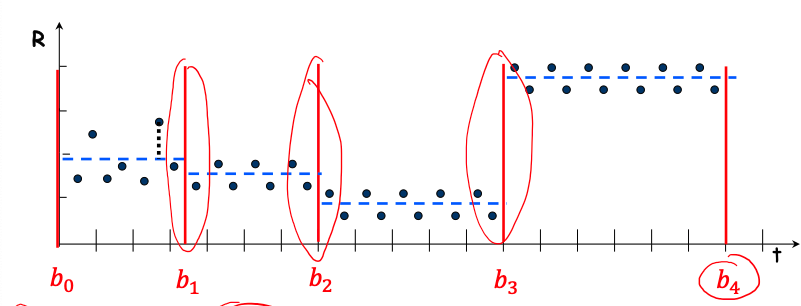
\includegraphics[width=1\textwidth]{images/sequenceseg.png}
        \end{center}
        
        A sequence $T = \set{t_1, \times, t_N}$. An ordered set of $N$ $d$-dimensional points $t_i \in \R^d$. A $K$-segmentation $S$ is a partition of $T$ into $K$ contiguous segments $\set{s_1, \times, s_k}$. Each segment $s \in S$ is represented by a single vector $\mu \in \R^d$. Which contains the representative of the segment (think centroid of cluster). The error $E(S)$ is the error of replacing individual points with representatives. There are a number of different representatives. The sum of squares error (SSE). \m{
            E(S) = \sum_{s \in S}\sum_{t \in s}(t - \mu_s)^2
        }
        Representative of segment $s$ with SSE is mean $\mu_s = \frac{1}{|s|}\sum_{t \in s}t$. 
        
        The \textbf{K-segmentation problem} is as follows: Given a sequence $T$ of length $N$ and a value $K$, find a $K$-segmentation $S = \set{s_1, \times, s_k}$ of $T$ such that the SSE error of $E$ is minimized. This is like $K$-means clustering, but points respect the order of the sequence. This makes it easier to sing.
        
        An observation: A $k$-segmentation of $S$ is defined as $K + 1$ boundary points $b_0, \times, b_K$. $b_0 = 0, b_k = N + 1$ are fixed, we only need to change the others. 
        
    \subsubsection{Solving $K$-segmentation as a dynamic programming problem}
        The $K$-segmentation can be solved optimally using a standard dynamic programming algorithm. 
        
        We will construct a solution to problems of smaller size. We will then build a solution bottom-up from smaller to larger instances. A rule is thumb is that optimization problems where order is involved can be solved optimally in polynomial time by dynamic programming. 
        
        Let us get some terminology in order. $T[1, i]$ subsequence $\set{t_1, \times, t_i}$ for $i \leq N$. $E(i, k)$ is the error of optimal segmentation of subsequence $T[1, i]$ with $k$ segments for $k \leq K$.
        
        Our DP recursion is \m{
            E(i, k) = \min_{k \leq j \leq i - 1}\set{E(j, k-1) + \sum_{i+1 \leq t \leq i}(t - \mu_{[j+1, i]})^2}
        }
        Where we minimize over all possible placements of the last boundary point. The $E$ is the error of the optimal segmentation of $T[1, j]$ with $k-1$ segments. The sum is the error of the $k$-th last segment $[j+1, i]$.
        
        We will store a table that we will fill from top to bottom, left to right. Bottom-right corner contains error of optimal $K$-segmentation. $A[k, i] = E(i, k)$
        
        \begin{center}
            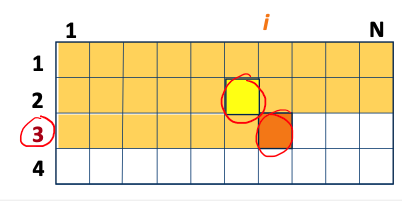
\includegraphics[width=1\textwidth]{images/table.png}
        \end{center}
         \begin{center}
            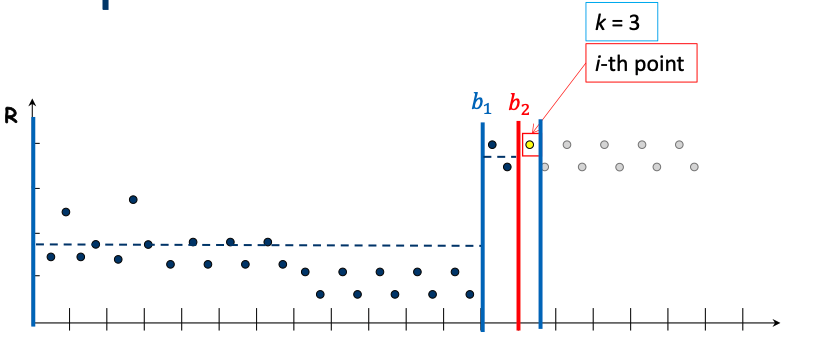
\includegraphics[width=1\textwidth]{images/placingk.png}
        \end{center}
        
        For example, in the example pictured, cell $A[3, i]$ stores the error of optimal $3$-segmentation of $T[1, i]$. In that cell (or somewhere else), we also store the position $i-3$ of the boundary, so we can trace back the segmentation. 
        
        The Dynamic Programming algorithm works as follows:
        \begin{itemize}
            \item For $i = 1$ to $N$ (Init first row), $A[1, i] = E(T[1, \dots, i])$. This is the error when everything is in one cluster.
            \item For $k = 1$ to $K$ (Init diagonal), $A[k, k] = 0$ This is the error when each point is in its own cluster
            \item For $k=2$ to $K$ and \begin{itemize}
                \item For $i = k + 1$ to $N$, $A[k, i] = \min_{j < i}\set{A[k-1, j] + E(T[j+1, \dots, i])}$
            \end{itemize}
        \end{itemize}
        To recover the actual segmentation, and not just the optimal cost, we also store the minimizing values $j$. 
        
        The complexity is 
        \begin{itemize}
            \item $NK$ cells to fill
            \item Computation per cell $E(i, k)$ has $O(N)$ boundaries to check per cell. $O(N)$ to compute second term per checked boundary
            \item $O(N^3K)$ in naive computation
            \item We can avoid the last $O(N)$ to observe that \m{
                \sum_{j+1 \leq t \leq i}(t - \mu_{[j+1, i]})^2 = \sum_{j+1 \leq t \leq i}t^2 - \frac{1}{i-j}(\sum_{j+1 \leq t \leq i})^2
            }
            \item That is, we can compute in constant time by precomputing partial sums. We precompute $\sum_{1 \leq t \leq i}t$ and $\sum_{i \leq t \leq i}t^2$
            \item Complexity is then $O(N^2K)$
        \end{itemize}
        
\subsubsection{Heuristics}
    There are a number of heuristics that we can use
    \begin{itemize}
        \item Top-down greedy (TD) is $O(NK)$. It introduces boundaries one at a time so that you can get the largest decrease in error until $K$ segments are created
        \item Bottom-up greedy (BU): $O(N \log N)$. Merge adjacent points each time selecting two points that cause the smallest increase in error until you have $K$ segments. 
        \item Local search heuristics: $O(NK)$ assign original breakpoints randomly then move them so as to reduce error
        \item Advanced local search: $O(NK)$. Collect candidate breakpoints by local search, apply DP on those breakpoints
    \end{itemize}
    
    Local search is a class of heuristic optimization algorithms that start with some solution and iteratively improves the solution with small local changes. Each solution has a set of neighboring solutions, we have a set of solutions that can be created with the allowed local changes. Usually we move to the best.
    
    Local search algorithms are surprisingly effective. For some problems, they yield optimal solutions or solutions with good approximation bounds.
    
    
    
\subsection{Finding similar items}
    Say we want to find near-neighbors in high-dimensional space. We each application, we need to define the Jaccard distance / similarity. The Jaccard similarity of two sets is the size of their intersection $sim(C_1, C_2) = |C_1 \cap C_2|/|C_1 \cup C_2|$. The Jaccard distance is then $d(C_1, C_2) = 1 - |C_1 \cap C_2|/|C_1 \cup C_2|$. 
    
    Say that we have a goal that we want to find near duplicate pairs. Say we have millions or billions of these, it becomes such a big problem that it may not fit into memory. There are $3$ essential steps for similar docs. 
    \begin{itemize}
        \item \textbf{Shingling:} Convert documents to sets
        \item \textbf{Min-hashing}: Convert large sets to short signatures, while preserving similarity
        \item \textbf{Locality-sensitive hashing:} Focus on pairs of signatures likely to be from similar documents
    \end{itemize}
    
    \begin{center}
        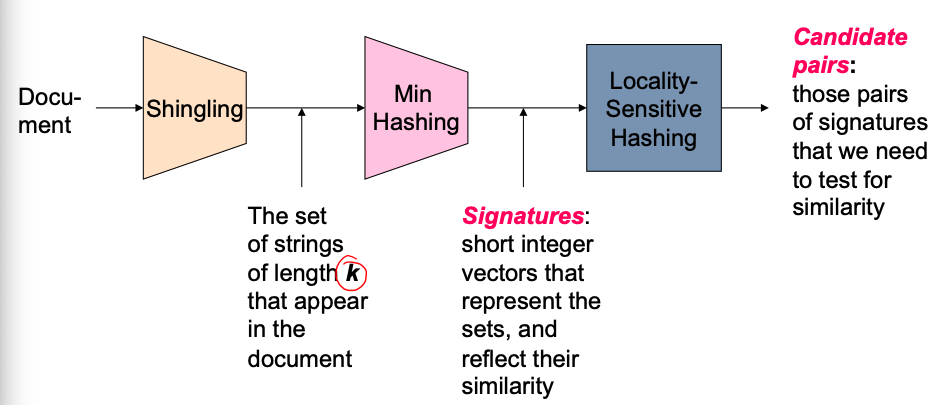
\includegraphics[width=1\textwidth]{images/documents.png}
    \end{center}
    
    \subsubsection{Shingling}
        We want to convert documents to sets, but we need to account for ordering of words. 
        
        A $k$-shingle (or $k$-gram) for a document is a sequence of $k$ tokens that appears in the document. Tokens can be characters, words or whatever. For example, for $k = 2$, document $D_1 = abcab$. The set of $2$-shingles is $S(D_1) = \set{ab, bc, ca}$. We can compress long shingles by hashing them. 
        
        We can represent a document by the set of hash values of its $k$-shingles. The idea is that two documents rarely appear to have shingles in common, when in fact only the hash values were shared. For example, for $S(D_1) = \set{ab, bc, ca}$. The hash is $h(D_1) = \set{1, 5, 7}$.
        
        We can also say that each document is a binary vector in the space of $k$-shingles. Each unique shingle is a dimension. They are very sparse. We can use Jaccard similarity.
        
        Our assumption is that documents have a lot of shingles in common if they are similar, even if it appears in a different order. You also need a $k$ large enough to have space enough.
        
    \subsubsection{Minhash / LSH}
        Computing pairwise Jaccard similarities for every pair would take too long. With \emph{MinHashing} we covnert large sets to short signatures while preserving similarity. 
        
        Many similarity problems can be formalized as finding subsets that have significant intersection. If we encode each set as a binary vector with one dimension per element in the universal set, then the intersection is a bitwise AND and set union a bitwise OR. 
        
        Say we create boolean matrices. The rows are elements (shingles), the columns are sets (documents). We place a $1$ in row $e$ and column $s$ iff $e$ is a member of s. Column similarity is the Jaccard similarity of the corresponding sets (Rows with value 1). In this matrix, each column is a document. 
        
        \begin{center}
            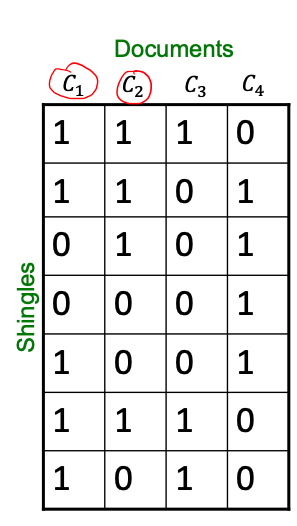
\includegraphics[width=1\textwidth]{images/shinglematrix.png}
        \end{center}
        
        We want to find similar columns while computing small signatures. Similarity of columns should be imply similarity of signatures. 
        
        The key idea is to hash each column to a small signature, $h(C)$ such that 
        \begin{itemize}
            \item $h(C)$ is small enough that the signature fits in RAM
            \item $sim(C_1, C_2)$ is the same as the similarity of signatures $h(C_1)$ and $h(C_2)$. 
        \end{itemize}
        Our goal is to find a hash function $h$ such that 
        \begin{itemize}
            \item $sim(C_1, C_2)$ is high, then with high prob the hashes are equal, otherwise then with high probability they are not equal
        \end{itemize}
        
        There is a suitable hash function for the Jaccard similarity: Min-hashing. We imagine the rows of the boolean matrix permuted under the random permutation $\pi$. We define our function $h_\pi(C)$ the index of the first (in the permuted order $\pi$) row in which column $C$ has value $1$.
        \m{
            h_\pi(C) = \min_\pi \pi(C)
        }
        We use several independent hash functions (permutations) to create a signature of a column. 
        
        The Min-hash property is that \m{
            Pr[h_\pi(C_1) = h_\pi(C_2)] = sim(C_1, C_2)
        }
        The reason why this works is that if we let $X$ be a doc (set of shingles), and $y \in X$ is a shingle. Then $Pr[\pi(y) = \min(\pi(X))] = 1/|X|$. It is equally likely that any $y \in X$ is mapped to the min element. Let $y$ be s.t that $\pi(y) = \min(\pi(C1 \cup C_2))$. Then either 
        \begin{itemize}
            \item $\pi(y) = \min(\pi(C_1))$ if $y \in C_1$ OR
            \item $\pi(y) = \min(\pi(C_2))$ if $y \in C_2$
        \end{itemize}
        Or one of the two columns had to have $1$ at position $y$. 
        So the probability thatboth are true is the probability that $y \in C_1 \cap C_2$. 
        
    We know that $Pr[h_\pi(C_1) = h_\pi(C_2)] = sim(C_1, C_2)$. We now generalize to multiple hash functions. The similarity of two signatures is the fraction of the hash functions in which they agree. Because of the minhash property, the similarity of columns is the same as the expected similarity of their signatures. 
    
    Say we pick $k = 100$ random permutations. We can think of $Sig(C)$ as a column vector. $Sig(C)[i] = \min(\pi_i(C))$. The sketch (or signature) of a document $C$ is small. We compressed long bit vectors into short signatures. 
    
    \subsubsection{Implementation trick}
        Permuting the rows is expensive. We can do row hashing. Say we pick $K = 100$ hash functions $k_i$. Ordering under $k_i$ gives a random row permutation. 
        
        The one-pass implementation is as follows: For each column $C$, and hash function, $k_i$ keep a "slot" for the min-hash value. We initialize $Sig(C)[i] = \infty$, then we scan rows looking for $1s$. Suppose row $j$ has $1$ in column $C$, then for each $k$, if $k_i(j) < Sig(C)[i]$, then $Sig(C)[i] = k_i(j)$. 
        
        How do we pick our hash function $h$? We can say $h_{a,b}(x) = ((ax+b) \mod p) \mod N$.
    
    \subsubsection{Locality Sensitive Hashing (LSH)}
        Wee focus on pairs of signatures likely to be from the same documents. 
        
        The goal is to find documents with Jaccard similarity at least $s$ for some threshold (such as $0.8$). The general idea behind LSH is to use a function $f(x,y)$ that tells if $x$ and $y$ is a candidate pair. That is a pair of elements whose similarity must be evaluated. 
        
        For min-hash matrices, we hash columns of signature matrix $M$ to many buckets. Each pair of documents that hashes into the same bucket is a candidate pair. 
        
        Pick a similarity threshold $s(0 < s <1)$. The columns of $x$ and $y$ of $M$ are a candidate pair if their signatures agree on at least a fraction $s$ of their rows. $M(i, x) = (Mi, y)$ for at least a fraction $s$ of $i$. 
        
        The idea is to hash columns of signature matrix $M$ several times. Similar columns should be likely to hash to the same bucket with high probability. 
        
        We partition $M$ into $b$ bands. These are vertical slices, with $r$ rows per band. We compute a signature on each band (subset of rows for each column). For each band we hash its portion of each column to a hash table with $k$ buckets. We want to make $k$ as large as possible. 
        
        Candidate column pairs are those that hash to the same bucket for $\geq 1$ band. Tune $b$ and $r$ to catch most similar pairs, but few non-similar pairs. 
        
        There are enough columns that enough buckets that columns are unlikely to hash tot he same bucket unless they are identical in a particular band. 
        
        LSH involves a tradeoff. The number of Min-hashes (Rows of $M$). The number of bands $b$ and the number of rows $r$ per band. To balance out false positives and negatives. 